\documentclass[a0]{a0poster}
\usepackage{tabularx}
\usepackage{palatino}
\usepackage{epsfig}
\usepackage{alltt}
\usepackage{graphicx,epsfig}
\usepackage{amsmath,color,amsthm,dsfont,amssymb,multirow}
\newcommand{\mybf}[1]{\mathbf{#1}}

\def\vlambdao{{\boldsymbol{\lambda}_1^T}}
\def\vlambdat{{\boldsymbol{\lambda}_2^T}} 
\def\vfo{\boldsymbol{f}_1}
\def\vft{\boldsymbol{f}_2}

\definecolor{DarkBlue}{rgb}{0.1,0.1,0.5}
\definecolor{Black}{rgb}{0.0,0.0,0.0}
\definecolor{Red}{rgb}{0.9,0.0,0.1}
\definecolor{DarkBlue2}{rgb}{0.00,0.08,0.6}
\definecolor{DarkRed2}{rgb}{0.6,0.00,0.08}
\definecolor{DarkGreen2}{rgb}{0.00,0.6,0.08}
%\newcommand{\yang}[1]{{\color{DarkBlue}\par{\Large\bf #1}\par}}
\newcommand{\yang}[1]{{\color{DarkBlue}\par{\bf #1}\par}}
\newcommand{\myBlue}[1]{{\color{DarkBlue}#1}}
\newcommand{\myGreen}[1]{{\color{DarkGreen2}#1}}

% For debugging, force all o/p to be on one page, even though it will overrun.
% Remove this to print final copy
% \textheight200in

\parindent=0pt
\newcommand{\rect}[2]{
\mbox{\begin{minipage}{#1}
\framebox[#1]{\rule{0pt}{#2}}
\vspace{-#2}
\vspace{-\baselineskip}
\vspace{-10pt}
\end{minipage}
}}

\def\m#1{{\tt #1}}
\def\v#1{{\bf #1}}
\newcommand{\colvec}[1]{\left( \begin{array}{c} #1 \end{array} \right)}
\newcommand{\awfwbox}[1]{\parbox{\textwidth}{\hspace*{\fill}#1\hspace*{\fill}}}
\newcommand{\epswide}[2]{\psfig{figure=#2,width=#1\textwidth}}
\newcommand{\epshigh}[2]{\psfig{figure=#2,height=#1\textwidth}}
\newcommand{\T}{{\cal T}}
\newtheorem{thm}{Theorem}

%\renewcommand{\paragraph}[1]{\vspace{1cm}\par{\Large\bf #1}\par}
\renewcommand{\paragraph}[1]{{\color{DarkRed2}\vspace{1cm}\par{\LARGE\bf #1}\par}}

\newcommand{\awfhline}{\rule{\textwidth}{1pt}}

\newlength{\colwidth}
%\setlength{\colwidth}{0.181\textwidth}
\setlength{\colwidth}{0.31\textwidth}

\newcommand{\col}[1]{
\fbox{
\begin{minipage}[t]{\colwidth}\raggedright\large
#1
\end{minipage}
}
}

\newcounter{elist}
\newenvironment{awfitemize}[1]{\begin{list}{#1}{
 \usecounter{elist}
 \setlength{\leftmargin}{2mm}
 \setlength{\labelwidth}{4mm}
 \setlength{\labelsep}{.1mm}
 \setlength{\itemindent}{0pt}
 \setlength{\rightmargin}{0pt}
}}{\end{list}}
% 
% \renewenvironment{itemize}{\awfitemize{$\bullet$\hfill}\setlength{\labelwidth}{2mm}}{\endawfitemize}
% \renewenvironment{enumerate}{\awfitemize{\arabic{elist}.}}{\endawfitemize}
% 

%%%%%%%%%%%%%%%%%%%%%%%%%%%%%%%%%%%%%%%%%%%%%%%%%%%%%%%%%%%%%%%%%%%%%%%%%%%%%
\newcommand{\awfp}[2]{{
\tiny\begin{tabular}{c}
\epsfysize=30mm\epsfbox{#1}\\
\hfill#2
\end{tabular}
\hspace{-1em}
}}

\begin{document}
\small
\thispagestyle{empty}
\rect{\textwidth}{\textheight}

\begin{tabularx}{\textwidth}{cXc}
\begin{minipage}{4in} 
\includegraphics[height=2.5in]{fig/SFU} \end{minipage}&
\centering \begin{minipage}{25in}
\begin{center}
{\color{DarkRed2}{\Huge\bf A Discriminative Latent Model of Object Classes and Attributes}}\\
{\color{DarkBlue}{\LARGE Yang Wang and Greg Mori}}\\
{\color{DarkBlue}{\large Vision and Media Lab, Simon Fraser University, Burnaby, BC, Canada}}\\
\end{center}
\end{minipage} &
\begin{minipage}{4in} 
\includegraphics[height=2.5in]{fig/vml} \end{minipage}
\end{tabularx}

%% Column 1
\begin{center}
\col{
\paragraph{Overview}
{\LARGE
\begin{itemize}
\item Joint modeling of object classes and (correlated) attributes
\item Use of word embedding to train Keras layers 
\item A general learning framework for classification with auxiliary labels
\end{itemize}
}

\vspace{2cm}



\awfhline

\paragraph{Model Formulation}
\begin{center}
\includegraphics[height=15in,width=12in]{fig/embedding_pic}
\end{center}

\vspace{0.1cm}

{\LARGE
{\bf Training data}: IMDB movie review. Labeled as negative and positive

\vspace{1cm}

{\bf Training algorithm for embedding }: Hierarchical softmax
\newline
{\bf Training algorithm for Keras layers }: softmax with stochastic gradient descent

}

}
%
\col{
\paragraph{Learning and Inference}
{\LARGE
{\bf Scoring}:  score(w,h) computes the compatibility of word w with the context h

\begin{eqnarray}
\mybf{P}(w_t | h)=softmax(score(w_t, h))\nonumber
&&\\=\frac{exp(socre(w_t,h)}{{ \sum_{w' in Vocab}{}}exp(score(w',h))}\nonumber
\end{eqnarray}

{\bf Learning with latent attributes}:
\begin{eqnarray}
&&\min_{\mybf{w},\xi}  \beta ||\mybf{w}||^{2}+\sum_{n=1}^{N}\xi^{(n)}\nonumber\\
&&{\rm s.t.} \max_{\mybf{h}}\mybf{w}^\top\Phi(\mybf{x}^{(n)},\mybf{h},y^{(n)})-\max_{\mybf{h}}\mybf{w}^\top\Phi(\mybf{x}^{(n)},\mybf{h},y) \nonumber\\
&&\ \ \ \ \ \ \geq \Delta(y,y^{(n)})-\xi^{(n)}, \forall n, \forall y\nonumber
\end{eqnarray}

%{\bf Learning with observed attributes}:
%\begin{eqnarray}
%&&\min_{\mybf{w},\xi} \beta||\mybf{w}||^{2}+\sum_{n=1}^{N}\xi^{(n)}\nonumber\\
%&&{\rm s.t.} \mybf{w}^\top\Phi(\mybf{x}^{(n)},\mybf{h}^{(n)},y^{(n)})-\max_{\mybf{h}}\mybf{w}^\top\Phi(\mybf{x}^{(n)},\mybf{h},y) \nonumber\\
%&&\ \ \ \ \ \ \geq \Delta(y,y^{(n)})-\xi^{(n)}, \forall n, \forall y\nonumber
%\end{eqnarray}

Another choice is to use the ground-truth attribute labels $\mybf{h}^n$ (i.e. learning with observed attributes).
} % LARGE

\awfhline
\paragraph{Attribute Relation Graph}
{\LARGE Running minimum spanning tree with $\mathrm{NormMI}(j,k)$ as the weight on the edge $(j,k)$.}


\awfhline
\paragraph{Other Loss Functions}
{\LARGE A simple modification of $\Delta$ will optimize different (training) errors.

{\bf Overall accuracy:}
\begin{eqnarray*}
\Delta_{\mathrm{0/1}}(y,y^{(n)})=\left\{ \begin{array}{ll}
    1 & \textrm{if $y\neq y^{(n)}$}\\
    0 & \textrm{otherwise}
    \end{array} \right.
\end{eqnarray*}

{\bf Mean per-class accuracy:}
\begin{eqnarray*}
\Delta_{\mathrm{new}}(y,y^{(n)})=\left\{ \begin{array}{ll}
    \frac{1}{m_p} & \textrm{if $y\neq y^{(n)}$ and $y^{(n)}=p$}\\
    0 & \textrm{otherwise}
    \end{array} \right.
\end{eqnarray*}
where $m_p$ is the number of training examples with class $p$.
}
} % col
%
\col{
\paragraph{Experiments}

\vspace{2cm}

\begin{center}
{\Large\bf a-Pascal dataset:}
\end{center}


{\large
\begin{center}
\begin{tabular}{|l||c|c|}
\hline
method & overall & mean per-class\\
\hline\hline
Our approach with $\Delta_{0/1}$ & {\bf 62.16} & {\bf 46.25} \\
Our approach with $\Delta_{\mathrm{new}}$ & {\bf 59.15} & {\bf 50.84}\\
\hline
SVM with $\Delta_{0/1}$ & 58.77 & 38.52\\
SVM with $\Delta_{\mathrm{new}}$ & 53.74 & 44.04\\
\hline
Farhadi et al. CVPR09~(base features+SVM) & 58.5 & 34.3\\
\hline
Farhadi et al. CVPR09~(best result) & 59.4 & 37.7\\
\hline
\end{tabular}
\end{center}
}

\vspace{2cm}

\begin{center}
{\Large\bf a-Yahoo dataset:}
\end{center}

\begin{center}
\begin{tabular}{cc}
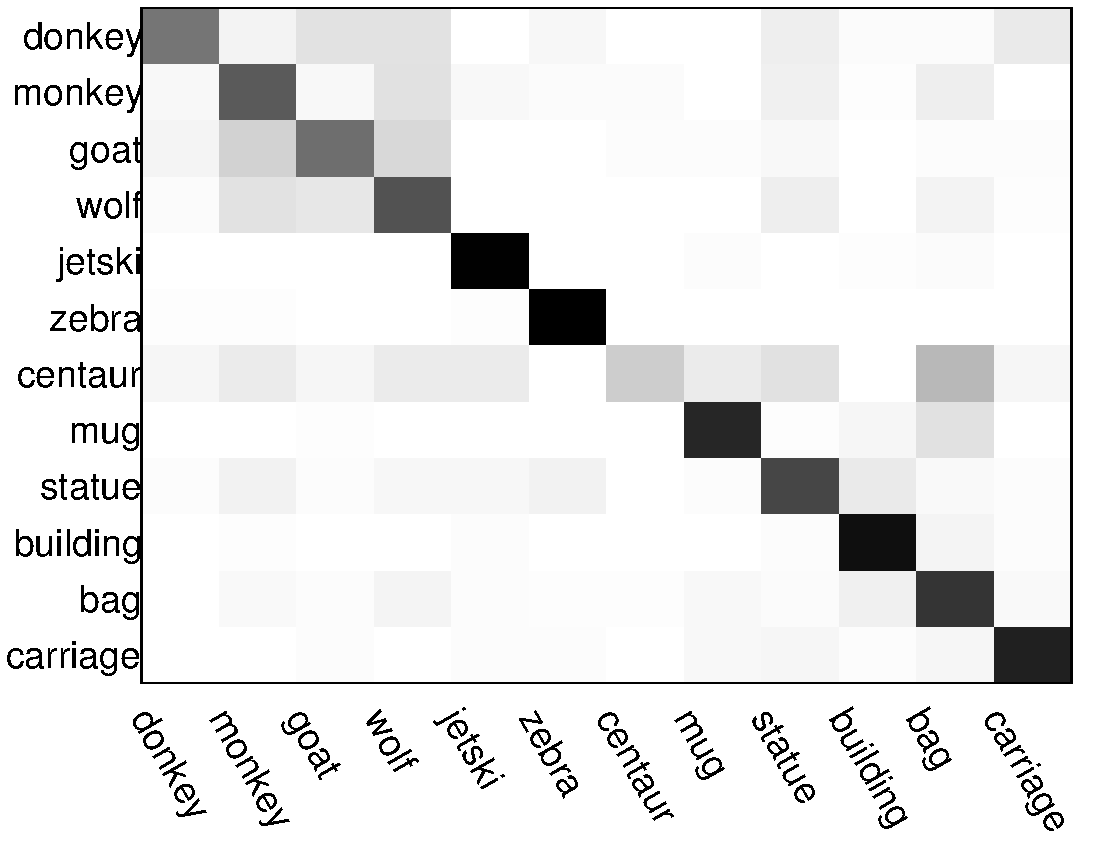
\includegraphics[height=8in, width=11in]{fig/yahoo_conf}&
\end{tabular}
\end{center}

{\Large
\begin{center}
\begin{tabular}{|l||c|c|}
\hline
method & overall & mean per-class\\
\hline\hline
Our approach with $\Delta_{0/1}$ & {\bf 78.67} & {\bf 71.45}\\
Our approach with $\Delta_{\mathrm{new}}$ & {\bf 79.88} & {\bf 73.31}\\
\hline
SVM with $\Delta_{0/1}$ & 74.43 & 65.96\\
SVM with $\Delta_{\mathrm{new}}$ & 74.51 & 66.74\\
\hline
\end{tabular}
\end{center}
}
}
%
\end{center}

\vfill
\begin{center}
{\color{DarkBlue}\LARGE \hspace{5cm}The 11th European Conference on Computer Vision, Heraklion, Crete, Greece, September 2010\hspace{5cm}}\\
\end{center}

\end{document}
